\section{Supplementary Material}

\subsection{Prolonged `Tap time' Following VR Glitches: Leveraging all trials for classification}

Subjecting all trials to the classification scheme, here we report results using the same analysis as in the behavioral part of the results section. Since we leveraged a 75\% to 25\% match to mismatch ratio this increased the amount of data significantly. `Tap time', the hand movement period from movement start to reaching the object, lasted on average .75s (SD = .15) in match- and .69s (SD = .15) in mismatch trials. 

We calculated the \textit{rate of change} in `tap time' as a metric of post-error slowing. Following match trials, `tap time' in the subsequent trial did not change, i.e. 0s (SD = .01). However, following mismatch trials, `tap time' was increased in the subsequent trial on average by .05s (SD = .04); this modulation was about 67 times more likely to occur under the model considering mismatch modulation than the null model (equivalent ${\chi}^2_{(1)} = 67.5, p<.001$), see figure \ref{setup_and_behavior}c.

\begin{figure}[!h]
  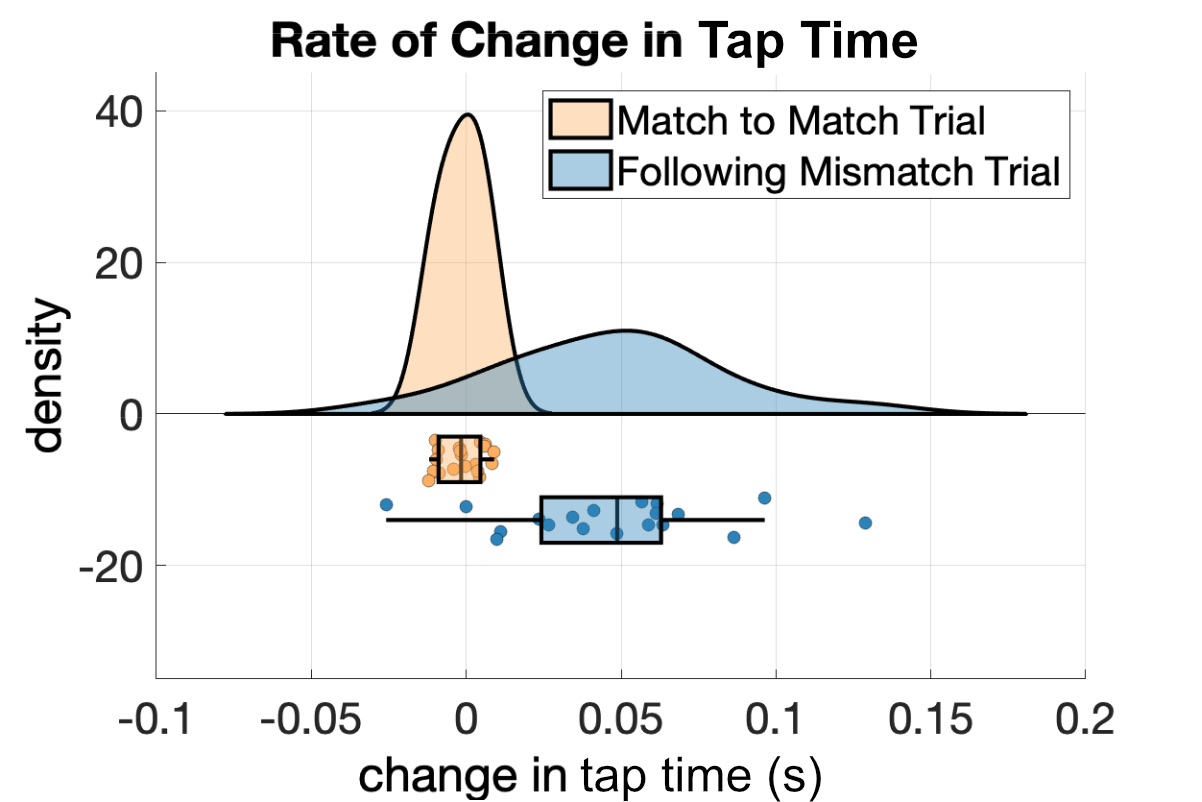
\includegraphics[width=.5\textwidth]{figures/rate_of_change_action_time_all_trials_.jpg}
  \caption{Distribution of \textit{rate of change} in `tap time' between two subsequent match trials and following a VR glitch. A dot represents the average per participant per condition. Here, all trial information is considered, maintaining unequal class sizes for match and mismatch conditions.}
  \label{behavior_supplements}
\end{figure}

Using the trial-to-trial adaptation in `tap time', trial classes (match/mismatch) were classified with an average within-subject classification accuracy across folds of $\sim$67\% (SD = 2.2), exceeding the significance threshold of the simulated chance level at $\sim$61\% (SD = 0.01, $t_{(18)} = 10.2, p < .001$.